\title{Classes of Inference}

{{navbar}}

\subsubsection{Classes of Inference}

Edward uses class inheritance to provide a hierarchy of inference
methods. Inference is broadly classified under three components:
variational inference, Monte Carlo, and exact inference.

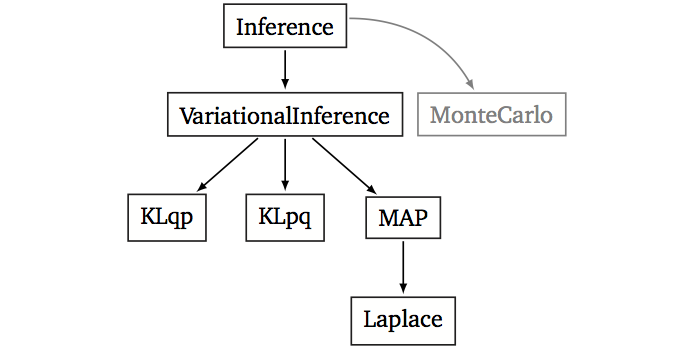
\includegraphics[width=700px]{/images/inference_structure.png}
{\small\textit{Dependency graph of inference methods.
Nodes are classes in Edward and arrows represent class inheritance.}}

Below we highlight how to use inference algorithms from each class.
We use the running example of a mixture model.

\subsubsection{Variational Inference}

In variational inference, the idea is to posit a family of approximating
distributions and to find the closest member in the family to the
posterior \citep{jordan1999introduction}.
We build the variational family in the graph.
The variational family has mutable
variables representing its parameters $\mathbf{\lambda}=\{\pi,\mu,\sigma\}$,
where
\begin{align*}
q(\beta;\mu,\sigma) &= \text{Normal}(\beta; \mu,\sigma), \\[1.5ex]
q(\mathbf{z};\pi) &= \text{Categorical}(\mathbf{z};\pi).
\end{align*}
\begin{lstlisting}[language=Python]
qbeta = Normal(mu=tf.Variable(tf.zeros([K, D])),
               sigma=tf.exp(tf.Variable(tf.zeros[K, D])))
qz = Categorical(logits=tf.Variable(tf.zeros[N, K]))

inference = ed.VariationalInference({beta: qbeta, z: qz}, data={x: x_train})
\end{lstlisting}
Given an objective function, variational inference optimizes the
factors with respect to \texttt{tf.Variable}s.

Specific variational inference algorithms inherit from
the \texttt{VariationalInference} class to define their own methods, such as a
loss function and gradient.
For example, we represent MAP estimation with
an approximating family of
\texttt{PointMass} random variables,
i.e., with all probability mass concentrated at a point.
\begin{lstlisting}[language=Python]
qbeta = PointMass(params=tf.Variable(tf.zeros([K, D])))
qz = PointMass(params=tf.Variable(tf.zeros(N)))

inference = ed.MAP({beta: qbeta, z: qz}, data={x: x_train})
\end{lstlisting}
\texttt{MAP}
inherits from \texttt{VariationalInference} and defines a loss
function and update rules; it leverages existing optimizers inside TensorFlow.

\subsubsection{Monte Carlo}

Monte Carlo approximates the posterior using samples
\citep{robert1999monte}. We represent Monte Carlo as inference where
the approximating family is an empirical distribution,
\begin{align*}
q(\beta; \{\beta^{(t)}\})
&= \frac{1}{T}\sum_{t=1}^T \delta(\beta, \beta^{(t)}), \\[1.5ex]
q(\mathbf{z}; \{\mathbf{z}^{(t)}\})
&= \frac{1}{T}\sum_{t=1}^T \delta(\mathbf{z}, \mathbf{z}^{(t)}).
\end{align*}
The parameters are $\mathbf{\lambda}=\{\beta^{(t)},\mathbf{z}^{(t)}\}$.
\begin{lstlisting}[language=Python]
T = 10000  # number of samples
qbeta = Empirical(params=tf.Variable(tf.zeros([T, K, D]))
qz = Empirical(params=tf.Variable(tf.zeros([T, N]))

inference = ed.MonteCarlo({beta: qbeta, z: qz}, data={x: x_train})
\end{lstlisting}
Monte Carlo
algorithms proceed by updating one sample $\beta^{(t)},\mathbf{z}^{(t)}$ at a time in the empirical
approximation.
Specific \glsunset{MC}\gls{MC} samplers determine the update rules;
they can leverage gradients and graph structure, where applicable.
Markov chain Monte Carlo does this sequentially to update
the current sample (index $t$ of \texttt{tf.Variable}s) conditional on
the last sample (index $t-1$ of the \texttt{tf.Variable}s).

\subsubsection{Exact Inference}

The approach also extends to exact inference. We are developing a
subpackage that does symbolic algebra on the deterministic and
stochastic nodes in the computational graph; this uncovers conjugacy
relationships between exponential-family random variables. This will
allow users to integrate out variables and automatically derive
classical Gibbs and mean-field updates \citep{bishop2006pattern} without
tedious algebraic manipulation.

\subsubsection{References}\label{references}
